\documentclass[dvisvgm,tikz,border=4pt]{standalone}
\usepackage{amsmath,amssymb}

\usetikzlibrary{arrows.meta,positioning,automata,shapes,shapes.misc,calc,decorations.pathmorphing,decorations.markings,angles,quotes,patterns,mindmap,matrix,knots,hobby,trees}
\tikzset{->-/.style={decoration={markings, mark=at position 0.5 with {\arrow{Stealth}}}, postaction={decorate}}}
\begin{document}
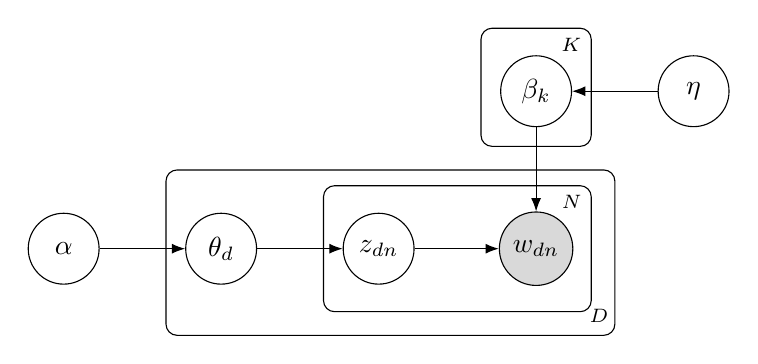
\begin{tikzpicture}[latent/.style={circle, draw, minimum size=9mm}, obs/.style={latent, fill=gray!30}, >=Latex]
\node[latent] (alpha) at (0,0) {$\alpha$};
\node[latent] (theta) at (2,0) {$\theta_d$};
\node[latent] (z) at (4,0) {$z_{dn}$};
\node[obs] (w) at (6,0) {$w_{dn}$};
\node[latent] (beta) at (6,2) {$\beta_k$};
\node[latent] (eta) at (8,2) {$\eta$};
\draw[->] (alpha) -- (theta); \draw[->] (theta) -- (z); \draw[->] (z) -- (w); \draw[->] (beta) -- (w); \draw[->] (eta) -- (beta);
\draw[rounded corners] (3.3,-0.8) rectangle (6.7,0.8) node[below left] {\scriptsize $N$};
\draw[rounded corners] (1.3,-1.1) rectangle (7,1.0) node[below left, yshift=-0pt] {};
\node at (6.8,-0.85) {\scriptsize $D$};
\draw[rounded corners] (5.3,1.3) rectangle (6.7,2.8) node[below left] {\scriptsize $K$};
\end{tikzpicture}
\end{document}
